\chapter{Basic Theory}
This chapter gives an overview of the basic ideas of the building blocks of this report. A review of probability distributions is done after which basic concepts from information theory which are relevant for the implementation are introduced.

\section{Probability Density Function}
The probability density function is an important probability function that will be useful for the implementation of this pre-thesis. We shall look at the probability density function (pdf) of the distributions used in the implementation.

\subsection{Uniform Distribution}
A process is said to be uniformly distributed if all the outcomes of the process are equally likely. For example, if we have a sample space $X$ of size n, that is uniformly distributed where \(0 < n  < \infty \) then the pdf is given as

\begin{equation}
p(x) =  \begin{cases} \frac{1}{n}  & \text{for all }  x \in  \mathcal{X}  \\  0 & \text{otherwise}\end{cases}
\end{equation}

\subsection{Gaussian Distribution}
The pdf of a gaussian distribution is given as 
\begin{equation}
p(x) = \frac{1}{\sqrt{2\pi\sigma_x^2}} \e^-\frac{(x-\mu_x)^2}{2\sigma_x^2}
\end{equation}
where $\sigma_x^2$ and $\mu_x$ represent the variance and mean respectively
\section{Concepts from Information Theory}
\subsection{Entropy}
Entropy is a measure of uncertainty in a given probability distribution. Assuming we have a collection of documents and a person wants to read a single document from the collection, we would like to guess the document chosen. Without any prior knowledge, every document is equally likely. We could assume that the longer documents have a higher probability while the shorter documents have a lower probability. From the assumption, if all the documents the same number of words, then they are all equally likely. Entropy vanishes as soon as the outcome of a process is certain. The entropy of a set is maximized when all elements in the set are equally likely.
\newline
Let $Y $ be a discrete random variable distributed according to $p(y)$. The entropy of $Y$ is defined by 
\begin{equation}
H(Y) = H[p(y)] = -\sum_y p(y) \log p(y)
\end{equation}

\subsection{Mutual Information}
Given a random variable $X$ with prior probability distribution $p(x)$ and some random variable $Y$ with probability distribution $p(y)$, the mutual information is the information common to $X$ and $Y$. Reconsidering our illustration of entropy above, assuming we also consider the distinct words in the collection of documents represented by $X$ and the collection of documents as $Y$. Here, we would not only consider the prior probability distributions but also the joint distribution $p(x, y)$ which indicates the probability that a random word in the collection is equal to $x \in  \mathcal{X}$ while the particular document is  $y \in  \mathcal{Y}$.
\newline
Mutual information is the reduction of uncertainty of $X$ due to the knowledge of $Y$ and also can be defined as the information gain about $X$ due to observation of $Y$.
\begin{equation}
I(X;Y) \equiv I[p(x, y)] = \sum_x \sum_y p(x, y) \log \frac{p(x, y)}{p(x)p(y)}
\end{equation}

\subsection{Channel Capacity}
Channel capacity is the maximum rate at which data can be transmitted through a channel. It can be obtained by maximizing the mutual information $I(X;Y)$  based on the statistical properties of the source signal.  According to the channel coding theorem of Shannon, reliable communication can only be achieved up to the channel capacity.

\begin{equation}
C = \sup_{Pr\{X\}} I( X; Y)
\end{equation}

\subsection{Kullback Leibler Divergence}
It is also known as the relative entropy and it is a measure of similarity between two distributions. It is not a symmetric measure as it is not commutative. Given two probability distributions $p_1(x)$ and $p_2(x)$, the Kullback Leibler (KL) divergence between them is defined as
\begin{equation}
D_{KL}(p_1||p_2 ) = \sum_x p_1(x) \log \frac{p_1(x)}{p_2(x)}
\end{equation}
Mutual Information between two distributions can be represented in terms of their Kullback Leibler Divergence. This relationship is given as
\begin{equation}
I(X;Y) = D_{KL}[p(x, y) | p(x)p(y)]
\end{equation}
\begin{figure}
\centering
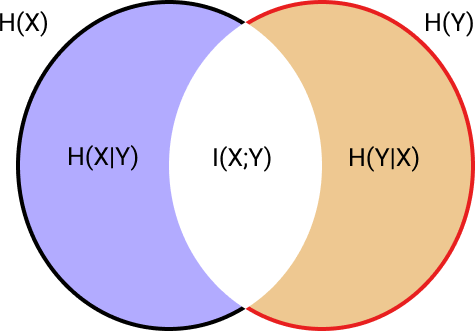
\includegraphics[scale=0.5]{Illustration_of_entropy}
\caption[Venn Diagram Illustrating Entropy and Mutual Information]{Venn Diagram Illustrating Entropy and Mutual Information: H(X) represents the entropy of X which in this case is the source signal. H(Y) represents the entropy of Y which is the sink. H(X|Y) is the entropy of X conditioned on Y. It is also called equivocation. It is the amount of information lost during transmission. H(Y|X) is known as the irrelevance i.e information not originating from the source. I(X;Y) which is the intersection of the two circles represents the mutual information }
\end{figure}
\subsection{Jensen Shannon Divergence}
This is another measure of distance between two distributions which is important for this topic. It is symmetric as opposed to KL divergence. The Jensen Shannon (JS) divergence between two probability distributions $p_1(x)$ and $p_2(x)$ is defined as
\begin{equation}
JS_{\Pi}[p_1, p_2] = \pi_1D_{KL}[p_1||\bar{p}] + \pi_2D_{KL}[p_2||\bar{p}]
\end{equation}
where \( \Pi = \{ \pi_1, \pi_2 \}, 0 < \pi_1, \pi_2 < 1, \pi_1 + \pi_2 = 1\) and  \(\bar{p} = \pi_1p_1 + \pi_2p_2\)
\subsection{Markov Chain}
Given 3 alphabets  $\mathcal{X}$, $\mathcal{Y}$ and $\mathcal{Z}$ with the relation $\mathcal{X}$ $\rightarrow$ $\mathcal{Y}$ $\rightarrow$ $\mathcal{Z}$,  since Z depends on Y, it cannot provide any "new" information about X, except the information already given by Y.
